\chapter{Conclusion and Future Directions}

\section{QTL Mapping with Causally Ambiguous Covariates}

In chapter 2, when using B as a mean or variance covariate for mapping A, we always assumed A was causally downstream of B, that no information flowed from B to A.
For example, no phenotype influences which batch, housing, or sex a mouse is.
In this setting, the value of including these covariates was clear.

Now, let's consider cases where the flow of causality is ambiguous.
What is the value in using B as a mean or variance covariate for mQTL and vQTL mapping?
WV and RC agree that using it as a variance covariate for mQTL mapping is probably a good thing -- gives weights that are more reflective of the true extent of residual variation.
But what about the other 3 possibilities?
There should be loads of literature on using it as a mean covariate for mQTL mapping -- trying to find some of that will be the next step for this section.


\centering
\begin{figure}
	\centering
	\begin{subfigure}{0.45\textwidth}
		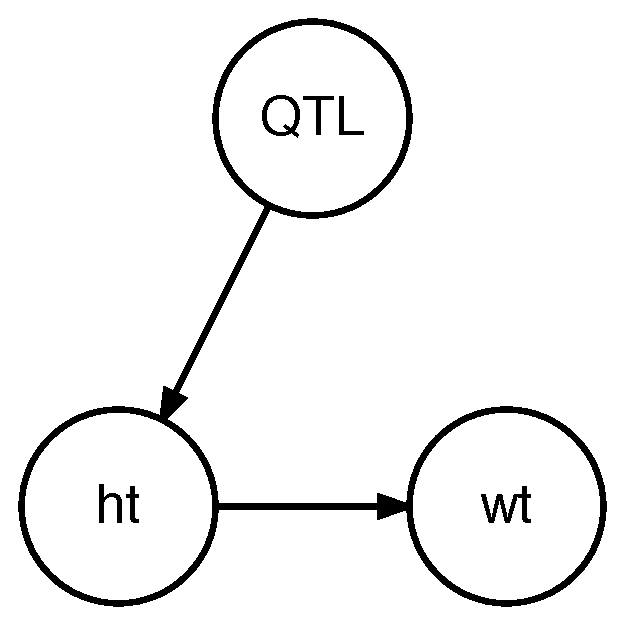
\includegraphics[width=0.8\linewidth]{images/graph_mm.pdf}
		\caption{Model MM: the QTL influences the mean of height and height influences the mean of weight.}
	\end{subfigure}\qquad
	\begin{subfigure}{0.45\textwidth}
		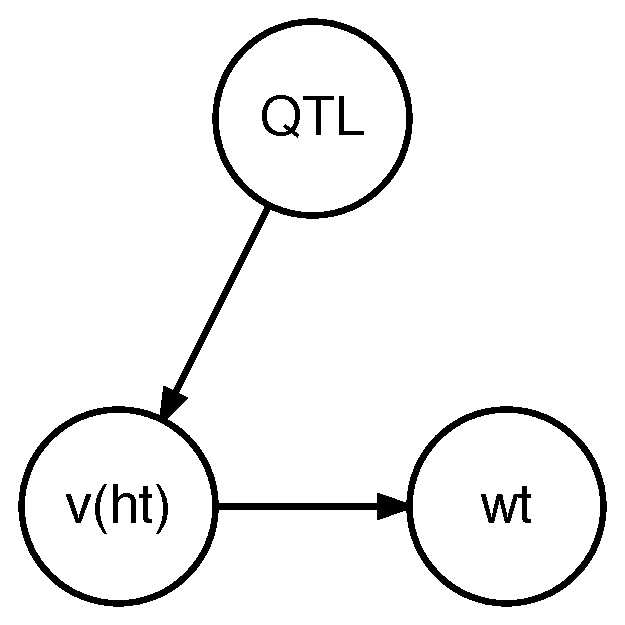
\includegraphics[width=0.8\linewidth]{images/graph_vm.pdf}
		\caption{Model VM: the QTL influences the variance of height and variance of height influences the mean of weight.}
	\end{subfigure}

	\vspace*{3em}
	
	\begin{subfigure}{0.45\textwidth}
		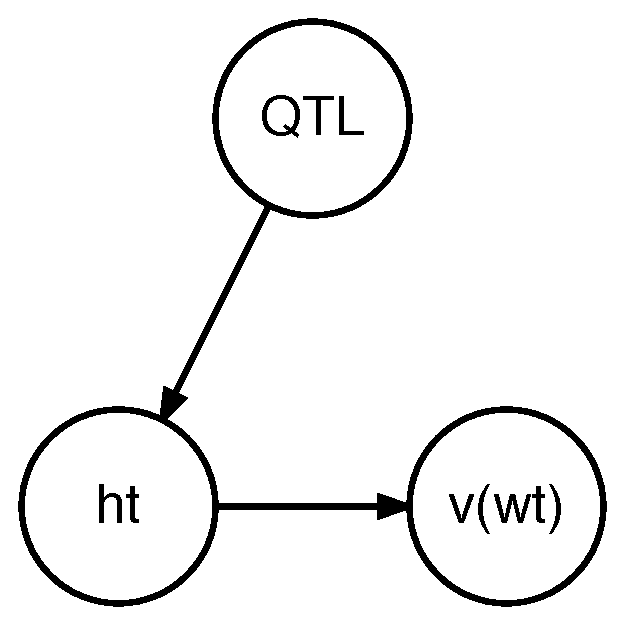
\includegraphics[width=0.8\linewidth]{images/graph_mv.pdf}
		\caption{Model MV: the QTL influences the mean of height and height influences the variance of weight.}
	\end{subfigure}\qquad
	\begin{subfigure}{0.45\textwidth}
		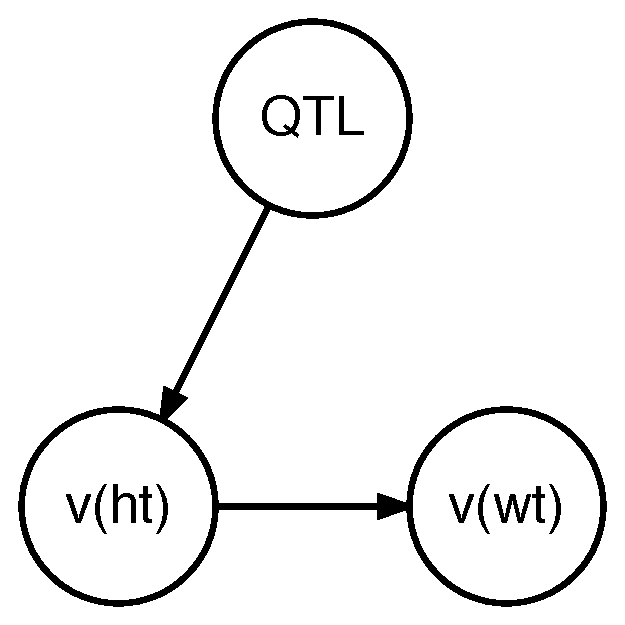
\includegraphics[width=0.8\linewidth]{images/graph_vv.pdf}
		\caption{Model VV: the QTL influences the variance of height and variance of height influences the variance of weight.}
	\end{subfigure}
\end{figure}
